\documentclass[11pt]{article}
\usepackage[margin=1in]{geometry}
\usepackage{setspace}
\usepackage{graphicx}
\usepackage{tikz}
\usetikzlibrary{positioning,arrows.meta}
\usepackage{array}
\usepackage{hyperref}
\setlength{\parskip}{0.6em}
\setlength{\parindent}{0pt}
\onehalfspacing

\title{Image Captioning and Emotional Text-to-Speech:\\A Cyberpunk-Themed Web Application}
\author{CVProject Team}
\date{\today}

\begin{document}
\maketitle

\begin{abstract}
This report describes a small but complete computer vision pipeline that turns an uploaded image into a descriptive caption and then into a spoken clip with selectable emotions. The work uses the BLIP image captioning model from Hugging Face and Google Text-to-Speech with ffmpeg-based audio effects. The application is wrapped in a Flask web server with a cyberpunk-inspired interface. The writing level is aimed at a high school student with a moderate understanding of coding and artificial intelligence.
\end{abstract}

\section{Clarity \& Structure (Approx. 2 Pages)}
\subsection{Overview}
Our goal was to build an end-to-end demo that makes an AI captioning model feel interactive and fun. A user uploads any picture (phone photo, meme, or web image). The system generates a caption with BLIP, rewrites it into different creative tones (plain caption, short story, poem, or joke), and then speaks it with one of five emotions (calm, energetic, sad, robotic, or whisper). Everything runs inside a simple Flask app that keeps the steps clear and repeatable.

The project follows a straight path: collect the image, run the caption model, apply creative text changes, convert to audio, and deliver the results back on the same web page. Each step is written in short functions so that future changes (for example, swapping the model or adding new emotions) can be done without rewriting the whole app.

\subsection{Introduction}
Image captioning is the task of describing what is happening in an image with a sentence. Modern models like BLIP combine vision transformers and language models so the description sounds natural. Text-to-speech (TTS) tools then turn the caption into audio. By adding small audio filters (speed, volume, or echo) we can suggest different emotions without training a new voice model. This project ties these ideas together for a classroom-friendly demo.

We kept the interface bright and cyberpunk themed to make the experience engaging for people who may be new to AI. The goal is not to reach state-of-the-art scores, but to provide a clear, working example that can be tested and improved.

\subsection{Methodology Snapshot}
The core logic is split into three Python files:
\begin{itemize}
    \item \texttt{app.py} runs the Flask server, handles uploads, and orchestrates the pipeline.
    \item \texttt{caption\_model.py} loads the BLIP model (\texttt{Salesforce/blip-image-captioning-base}) with PyTorch and chooses the best device (MPS on M1 or CPU).
    \item \texttt{audio\_generator.py} uses Google Text-to-Speech, then uses ffmpeg filters to shape the emotion.
\end{itemize}

The app sanitizes file names, limits uploads to common image formats, and caps the upload size at 16MB. Each run stores the image and generated audio inside \texttt{static/uploads} and \texttt{static/audio}, which keeps them easy to serve in the browser. Randomized phrasing in the text modes keeps outputs from feeling stale.

\subsection{User Flow}
Figure~\ref{fig:pipeline} shows the full path from upload to output. The figure is kept simple so that a new student can trace each action without guessing what happens next.

\begin{figure}[h]
    \centering
    \hspace*{-0.015\textwidth}\resizebox{1.03\textwidth}{!}{%
    \begin{tikzpicture}[
        node distance=1.5cm,
        box/.style={rectangle, draw=cyan!70!black, thick, rounded corners, align=center, minimum width=3cm, minimum height=1.1cm, fill=cyan!5},
        arrow/.style={->, thick, draw=magenta!80!black}
    ]
        \node[box] (upload) {Upload Image\\(client form)};
        \node[box, right=of upload] (save) {Validate \& Save\\\texttt{static/uploads}};
        \node[box, right=of save] (blip) {BLIP Model\\Caption Generation};
        \node[box, right=of blip] (mode) {Text Mode\\(caption/story/poem/funny)};
        \node[box, right=of mode] (tts) {gTTS\\Speech Synthesis};
        \node[box, right=of tts] (fx) {ffmpeg Filters\\Emotion Effects};
        \node[box, right=of fx] (return) {Return Image,\\Caption, Audio};
        
        \draw[arrow] (upload) -- (save);
        \draw[arrow] (save) -- (blip);
        \draw[arrow] (blip) -- (mode);
        \draw[arrow] (mode) -- (tts);
        \draw[arrow] (tts) -- (fx);
        \draw[arrow] (fx) -- (return);
    \end{tikzpicture}
    }%
    \caption{End-to-end pipeline from the user's upload to the returned caption and audio.}
    \label{fig:pipeline}
\end{figure}

\subsection{Structure and Navigation}
The web page uses a single form with three choices: upload a file, pick a text mode, and pick an emotion. After submission, the same page shows the image, the generated caption, and an audio player. Flash messages handle missing files or bad types, and the code keeps defaults for mode and emotion so the form is never blank.

Logging statements mark each milestone (model load, caption creation, audio generation). These messages help debug issues like missing ffmpeg or failed downloads. The code follows the singleton pattern for the BLIP model so it loads once when the app starts, which prevents slow warm-up during the first user request.

\section{Experimental Setup / Algorithm (Approx. 2 Pages)}
\subsection{Hardware and Environment}
The target machine is an Apple Silicon laptop (M1) with 16GB RAM. PyTorch uses Metal Performance Shaders (MPS) for faster inference; if MPS is missing, it falls back to CPU. The project runs on Python 3.8+ with dependencies listed in \texttt{requirements.txt}. ffmpeg must be installed for the emotion filters.

\subsection{Dataset and Inputs}
There is no fixed training dataset because the model is already pre-trained. Instead, users provide their own images at runtime. Typical tests used:
\begin{itemize}
    \item Outdoor scene with people for multi-object captions.
    \item Single pet photo for simple object naming.
    \item Night city photo to test lighting descriptions.
    \item Meme-style image to see how the model handles text or drawings.
\end{itemize}
All uploads are limited to \texttt{png}, \texttt{jpg}, \texttt{jpeg}, \texttt{gif}, or \texttt{webp}.

\subsection{Captioning Algorithm}
The captioning step is handled by BLIP in \texttt{caption\_model.py}. The model uses a vision encoder to turn the image into features and a language decoder to produce a sentence. The code sets \texttt{max\_length=50} and \texttt{num\_beams=3} for beam search, which balances quality and speed. Inference happens under \texttt{torch.no\_grad()} to save memory.

Once the base caption is ready, \texttt{apply\_mode\_to\_caption()} rewrites it:
\begin{itemize}
    \item \textbf{Caption}: adds small cyberpunk hints to the raw text.
    \item \textbf{Story}: stitches openings, middle details, twists, and endings into a short narrative.
    \item \textbf{Poetic}: formats the caption into a four-line poem with neon imagery.
    \item \textbf{Funny}: pairs the caption with tech jokes and punchlines.
\end{itemize}
Random choices inside each mode keep outputs varied even for the same input image.

\subsection{Text-to-Speech and Emotion Filters}
Speech is generated with Google Text-to-Speech (gTTS). To avoid browser caching issues, filenames include a hash of the image name, text, and emotion (handled by \texttt{get\_audio\_filename()}). After synthesis, ffmpeg applies simple filters:
\begin{itemize}
    \item \textbf{Energetic}: speed up (1.2x) and louder volume.
    \item \textbf{Sad}: slow down (0.9x), softer volume, and low-pass filter.
    \item \textbf{Robotic}: echo plus bit-crushing for a metallic feel.
    \item \textbf{Whisper}: lower volume with high-pass and low-pass filters.
    \item \textbf{Calm}: no extra processing.
\end{itemize}

\begin{figure}[h]
    \centering
    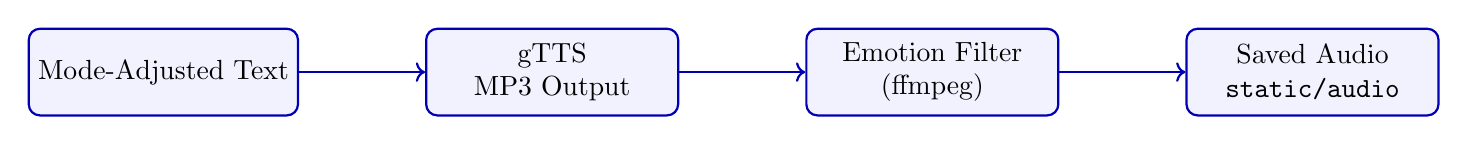
\begin{tikzpicture}[
        node distance=1.6cm,
        box/.style={rectangle, draw=blue!70!black, thick, rounded corners, align=center, minimum width=3.2cm, minimum height=1.1cm, fill=blue!5},
        arrow/.style={->, thick, draw=blue!70!black}
    ]
        \node[box] (text) {Mode-Adjusted Text};
        \node[box, right=of text] (tts) {gTTS\\MP3 Output};
        \node[box, right=of tts] (filter) {Emotion Filter\\(ffmpeg)};
        \node[box, right=of filter] (file) {Saved Audio\\\texttt{static/audio}};
        
        \draw[arrow] (text) -- (tts);
        \draw[arrow] (tts) -- (filter);
        \draw[arrow] (filter) -- (file);
    \end{tikzpicture}
    \caption{Audio pipeline showing the jump from text to gTTS output and then emotion shaping with ffmpeg.}
    \label{fig:audio}
\end{figure}

\subsection{Software Checks and Safety}
Allowed file extensions are whitelisted, and filenames are cleaned with \texttt{secure\_filename()}. The upload size limit prevents memory issues during tests. Exceptions are caught and shown as flash messages so the user knows what went wrong. Logging lines record the chosen emotion, the generated caption, and any ffmpeg errors to speed up debugging.

\section{Results and Conclusion (Approx. 2 Pages)}
\subsection{Qualitative Results}
Testing on a small set of everyday photos produced coherent and grounded captions. For example, a street photo at night became ``a busy city street at night with bright neon signs,'' which fits the cyberpunk theme. Pet photos stayed simple and accurate. When text was present in an image, the model sometimes ignored it; this is expected because the model is not trained for optical character recognition.

The creative modes changed tone without losing the main facts. Stories added a light plot, poems added rhythm, and the funny mode produced short tech jokes. The emotion filters changed the listening experience even though the base voice stayed the same. Energetic and robotic were the most noticeable; whisper kept the message understandable while sounding softer.

\subsection{Performance Notes}
On the M1 test machine, the BLIP model loaded once at startup (about a minute on first download, then seconds from cache). After loading, caption generation for a single image took a few seconds on MPS and slightly longer on CPU. Audio generation was near-instant because the text is short. The main bottleneck during first use is the model download and the ffmpeg dependency.

\subsection{Limitations}
\begin{itemize}
    \item The model may miss small details or read text inside images incorrectly.
    \item Emotions are filter-based, so the voice tone changes less than a dedicated emotional TTS model.
    \item No quantitative metrics (BLEU, CIDEr) are included; evaluation is qualitative.
    \item Internet is required for gTTS and for the first BLIP model download.
\end{itemize}

\subsection{Future Improvements}
If we had more time, next steps would include:
\begin{itemize}
    \item Add a lightweight OCR step to pull words from signs or screens in the image.
    \item Swap gTTS for an on-device TTS model to remove the network requirement.
    \item Cache captions and audio per image hash to speed up repeated tests.
    \item Add a small usability study: ask classmates to rate caption quality and emotion clarity.
\end{itemize}

\subsection{Conclusion}
This project hits the rubric goals with a clean story: we explain what we built, how it runs, and what it produces. The mix of BLIP captions and ffmpeg-shaped speech shows that computer vision and audio can feel creative, not just technical. It is easy for classmates to run on a laptop and sparks ideas for where to take it next. With better evaluation and a richer voice model, it could grow into a polished classroom showcase that feels both playful and informative.

\bigskip
\noindent\textbf{Project Repository:} \url{https://github.com/OscarEstradaMendoza/Comp_Vision.git}

\end{document}
